\subsection*{The Inverse of a Function}
In previous mathematics courses, we learned that the exponential function (with base  $e$) and the natural logarithm function are inverses of each other.  This was often expressed as follows:
\begin{align*}
&\text{For each } x \in \R \text{ with } x > 0 \text{ and for each } y \in \R, \\
&y = \ln x \text{ if and only if } x = e^y.
\end{align*}
Notice that this means that $x$ is the input and $y$ is the output for the natural logarithm function if and only if $y$ is the input and $x$ is the output for the exponential function.  In essence, the inverse function (in this case, the exponential function) reverses the action of the original function (in this case, the natural logarithm function).  In terms of ordered pairs (input-output pairs), this means that if  $( {x, y} )$ is an ordered pair for a function, then  $( {y, x} )$ is an ordered pair for its inverse.  This idea of reversing the roles of the first and second coordinates is the basis for our definition of the inverse of a function.
%\begin{itemize}
%\item For each  $x \in \R$,  if  $y = e^x $, then  $\ln y = x$.
%
%\item For each  $x \in \R$ such that  $x > 0$,  if  $y = \ln x$, then  $e^y  = x$.
%\end{itemize}
%
%In each case,  when  $x$  is the input for one of the functions,  $y$  is the output.  If  $y$  is used as the input for the other function, then this produces  $x$  as the output.   In essence, the inverse function reverses the action of the original function.  In terms of ordered pairs (input-output pairs), this means that if  $( {x, y} )$ is an ordered pair for a function, then  $( {y, x} )$ is an ordered pair for its inverse.  This idea of reversing the roles of the first and second coordinates is the basis for our definition of the inverse of a function.
%
\begin{defbox}{inversefunction}{Let  $f\x A \to B$  be a function.  The \textbf{inverse of}
\index{inverse of a function}%
\index{function!inverse of}%
  $\boldsymbol{f}$\!, denoted by  $f^{ - 1} $,
\label{sym:finverse} is the set of ordered pairs  
$\left\{ { {( {b, a} ) \in B \times A} \mid f( a ) = b} \right\}$.  That is,
\[
f^{ - 1}  = \left\{ { {( {b, a} ) \in B \times A} \mid f( a ) = b} \right\}\!.
\]
If we use the ordered pair representation for  $f$\!, we could also write
\[
f^{ - 1}  = \left\{ { {( {b, a} ) \in B \times A} \mid ( {a, b} ) \in f} \right\}\!.
\]
}
\end{defbox}
%
Notice that this definition does not state that  $f^{ - 1} $  is a function.  It is simply a subset of  $B \times A$.  After we study the material in Chapter~\ref{C:equivrelations}, we will say that this means that  $f^{ - 1}$ is a \textbf{relation} from  $B$  to  $A$.  This fact, however, is not important to us now.  We are mainly interested in the following question:

\begin{center}
\fbox{
\parbox{4.5in}{{\textbf{Under what conditions will the inverse of the function  $\boldsymbol{f\x A \to B}$  be a function from  $B$  to  $A$?}}
}}
\end{center}

\begin{prog}[\textbf{Exploring the Inverse of a Function}] \label{prog:exploringinverse} \hfill \\
Let  $A = \left\{ {a, b, c} \right\}$, $B = \left\{ {a,b,c,d} \right\}$, and 
$C = \left\{ {p, q, r} \right\}$.  Define
\begin{center}
\begin{tabular}{c | c | c}
$f\x A \to C$ by &  $g\x A \to C$ by &  $h\x B \to C$ by \\
$f( a ) = r $  &  $g( a ) = p $  &  $h( a ) = p $ \\
$f( b ) = p $  &  $g( b ) = q $  &  $h( b ) = q $ \\
$f( c ) = q $  &  $g( c ) = p $  &  $h( c ) = r $ \\
                          &                            &  $h( d ) = q $
\end{tabular}
\end{center}
\begin{enumerate}
\item Draw an arrow diagram for each function.  \label{A:exploringinverse1}

\item Determine the inverse of each function as a set of ordered pairs.

\item \begin{enumerate} \item Is  $f^{ - 1} $ a function from  $C$  to  $A$?  Explain.

  \item Is  $g^{ - 1} $ a function from  $C$  to  $A$?  Explain.

  \item Is  $h^{ - 1} $  a function from  $C$  to  $B$?  Explain.
\end{enumerate}
\label{A:exploringinverse3}

\item Draw an arrow diagram for each inverse from  Part~(\ref{A:exploringinverse3}) that is a function.  Use your existing arrow diagram from Part~(\ref{A:exploringinverse1}) to draw this arrow diagram.

\item Make a conjecture about what conditions on a function  $F\x S \to T$ will ensure that its inverse is a function  from  $T$  to  $S$.
\end{enumerate}
\end{prog}
%\hbreak
%
We will now consider a general argument suggested by the explorations in Progress 
Check~\ref{prog:exploringinverse}.  By definition, if  $f\x A \to B$  is a function, then  
$f^{ - 1} $ is a subset of  $B \times A$.  However,  $f^{ - 1} $ may or may not be a function from  $B$  to  $A$.  For example, suppose that  $s, t \in A$ with  $s \ne t$  and  
$f( s ) = f( t )$.  This is represented in 
Figure~\ref{fig:inversenotfunction}.

\begin{figure}[h]
\begin{center}
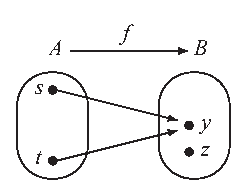
\includegraphics{figps-noinverse.eps}
\caption{The Inverse Is Not a Function} \label{fig:inversenotfunction}
\end{center}
\end{figure}


In this case, if we try to reverse the arrows, we will not get a function from  $B$  to  $A$.  This is because  $( {y, s} ) \in f^{ - 1} $  and  
$( {y, t} ) \in f^{ - 1} $ with  $s \ne t$.  Consequently,  $f^{ - 1} $  is not a function.  This suggests that when  $f$  is not an injection, then  $f^{ - 1} $  is not a function.  

Also, if  $f$  is not a surjection, then there exists a  $z \in B$ such that  
$f( a ) \ne z$ for all  $a \in A$, as in the diagram in 
Figure~\ref{fig:inversenotfunction}.  In other words, there is no ordered pair in  $f$  with  $z$  as the second coordinate.  This means that there would be no ordered pair in  
$f^{ - 1} $  with  $z$  as a first coordinate.  Consequently, $f^{ - 1} $  cannot be a function from  $B$  to  $A$.

This motivates the statement in Theorem~\ref{T:inverseandbijection}.  In the proof of this theorem, we will frequently change back and forth from the input-output representation of a function and the ordered pair representation of a function.  The idea is that if  $G\x S \to T$  is a function, then for  
$s \in S$  and  $t \in T$\!,
\[
G( s ) = t  \text{ if and only if }  ( {s, t} ) \in G.
\]
When we use the ordered pair representation of a function, we will also use the ordered pair representation of its inverse.  In this case, we know that
\[
( {s, t} ) \in G\text{ if and only if }( {t, s} ) \in G^{ - 1}. 
\]
%\hbreak
%
\begin{theorem} \label{T:inverseandbijection}
Let  $A$  and  $B$  be nonempty sets and let  $f\x A \to B$.  The inverse of  $f$ is a function from  $B$  to  $A$  if and only if  $f$  is a bijection.  
%(That is,  $f$  is both one-to-one and onto.)
\end{theorem}
%
\begin{myproof}
Let  $A$  and  $B$  be nonempty sets and let  $f\x A \to B$.  We will first assume that  $f$  is a bijection and prove that  $f^{ - 1} $ is a function from  $B$  to  $A$.  To do this, we will show that  $f^{ - 1} $ satisfies the two conditions of Theorem~\ref{T:functionasordered}.

We first choose  $b \in B$.  Since the function  $f$  is a surjection,  there exists an  
$a \in A$  such that  $f( a ) = b$.  This implies that  
$( {a, b} ) \in f$ and hence that  $( {b, a} ) \in f^{ - 1} $.  Thus, each element of  $B$  is the first coordinate of an ordered pair in  $f^{ - 1} $, and hence  
$f^{ - 1} $  satisfies the first condition of Theorem~\ref{T:functionasordered}.

To prove that  $f^{ - 1} $  satisfies the second condition of Theorem~\ref{T:functionasordered}, we must show that each element of  $B$  is the first coordinate of exactly one ordered pair in  $f^{ - 1} $.  So let  $b \in B$, $a_1 , a_2  \in A$
 and assume that  
\[
( {b, a_1 } ) \in f^{ - 1} \text{ and } ( {b, a_2 } ) \in f^{ - 1} .
\]
This means that  $( {a_1 , b} ) \in f$ and  $( {a_2 , b} ) \in f$.  We can then conclude that
\[
f( {a_1 } ) = b\text{ and }f( {a_2 } ) = b.
\]
But this means that  $f( {a_1 } ) = f( {a_2 } )$.  Since  $f$  is a bijection, it is an injection, and we can conclude that  $a_1  = a_2 $.  This proves that  $b$  is the first element of only one ordered pair in  $f^{ - 1} $.  Consequently, we have proved that  $f^{ - 1} $  satisfies both conditions of Theorem~\ref{T:functionasordered} and hence that  $f^{ - 1} $  is a function from  $B$  to  $A$.
\vskip6pt

We now assume that  $f^{ - 1} $  is a function from  $B$  to  $A$ and prove that  $f$  is a bijection. First, to prove that  $f$  is an injection, we assume that  $a_1 , a_2  \in A$ and that $f( {a_1 } ) = f( {a_2 } )$.  We wish to show that  $a_1  = a_2 $.  If we let  $b = f( {a_1 } ) = f( {a_2 } )$, we can conclude that
\[
( {a_1 , b} ) \in f \text{ and }( {a_2 , b} ) \in f.
\]
But this means that  
\[
( {b, a_1 } ) \in f^{ - 1} \text{ and }( {b, a_2 } ) \in f^{ - 1}. 
\]
Since we have assumed that  $f^{ - 1} $ is a function, we can conclude that  $a_1  = a_2 $.  Hence,  $f$  is an injection.

Now to prove that  $f$  is a surjection, we choose  $b \in B$ and will show that there exists an  $a \in A$ such that  $f( a ) = b$.  Since  $f^{ - 1} $  is a function,  $b$  must be the first coordinate of some ordered pair in  $f^{ - 1} $.  Consequently, there exists an  
$a \in A$  such that
\[
( {b, a} ) \in f^{ - 1} .
\]
Now this implies that  $( {a, b} ) \in f$ and hence that  $f( a ) = b$.  This proves that  $f$  is a surjection.  Since we have also proved that  $f$  is an injection, we conclude that  $f$  is a bijection.
\end{myproof}
\hbreak

\endinput
